\documentclass[11pt]{article}
\usepackage{amsmath, amssymb, amsthm}
\usepackage{xcolor}
\usepackage[most]{tcolorbox}
\usepackage{geometry}
\geometry{margin=1.5cm}
\usepackage{graphicx}
\usepackage{enumitem}
\usepackage{tikz}
\usepackage{tikz-3dplot}
\usepackage{multicol}
\usepackage{lmodern}
\usepackage{setspace}
\usepackage{titlesec}
\usepackage{fancyhdr}
\usetikzlibrary{arrows.meta}
\usepackage{array}
\usepackage{booktabs}
\usepackage{hyperref}


\setlength{\parindent}{0pt}
\newtcolorbox{remarkbox}{colback=red!5!white,colframe=red!75!black,title=Remark}
\begin{document}

\begin{figure}[!ht]
    \centering
    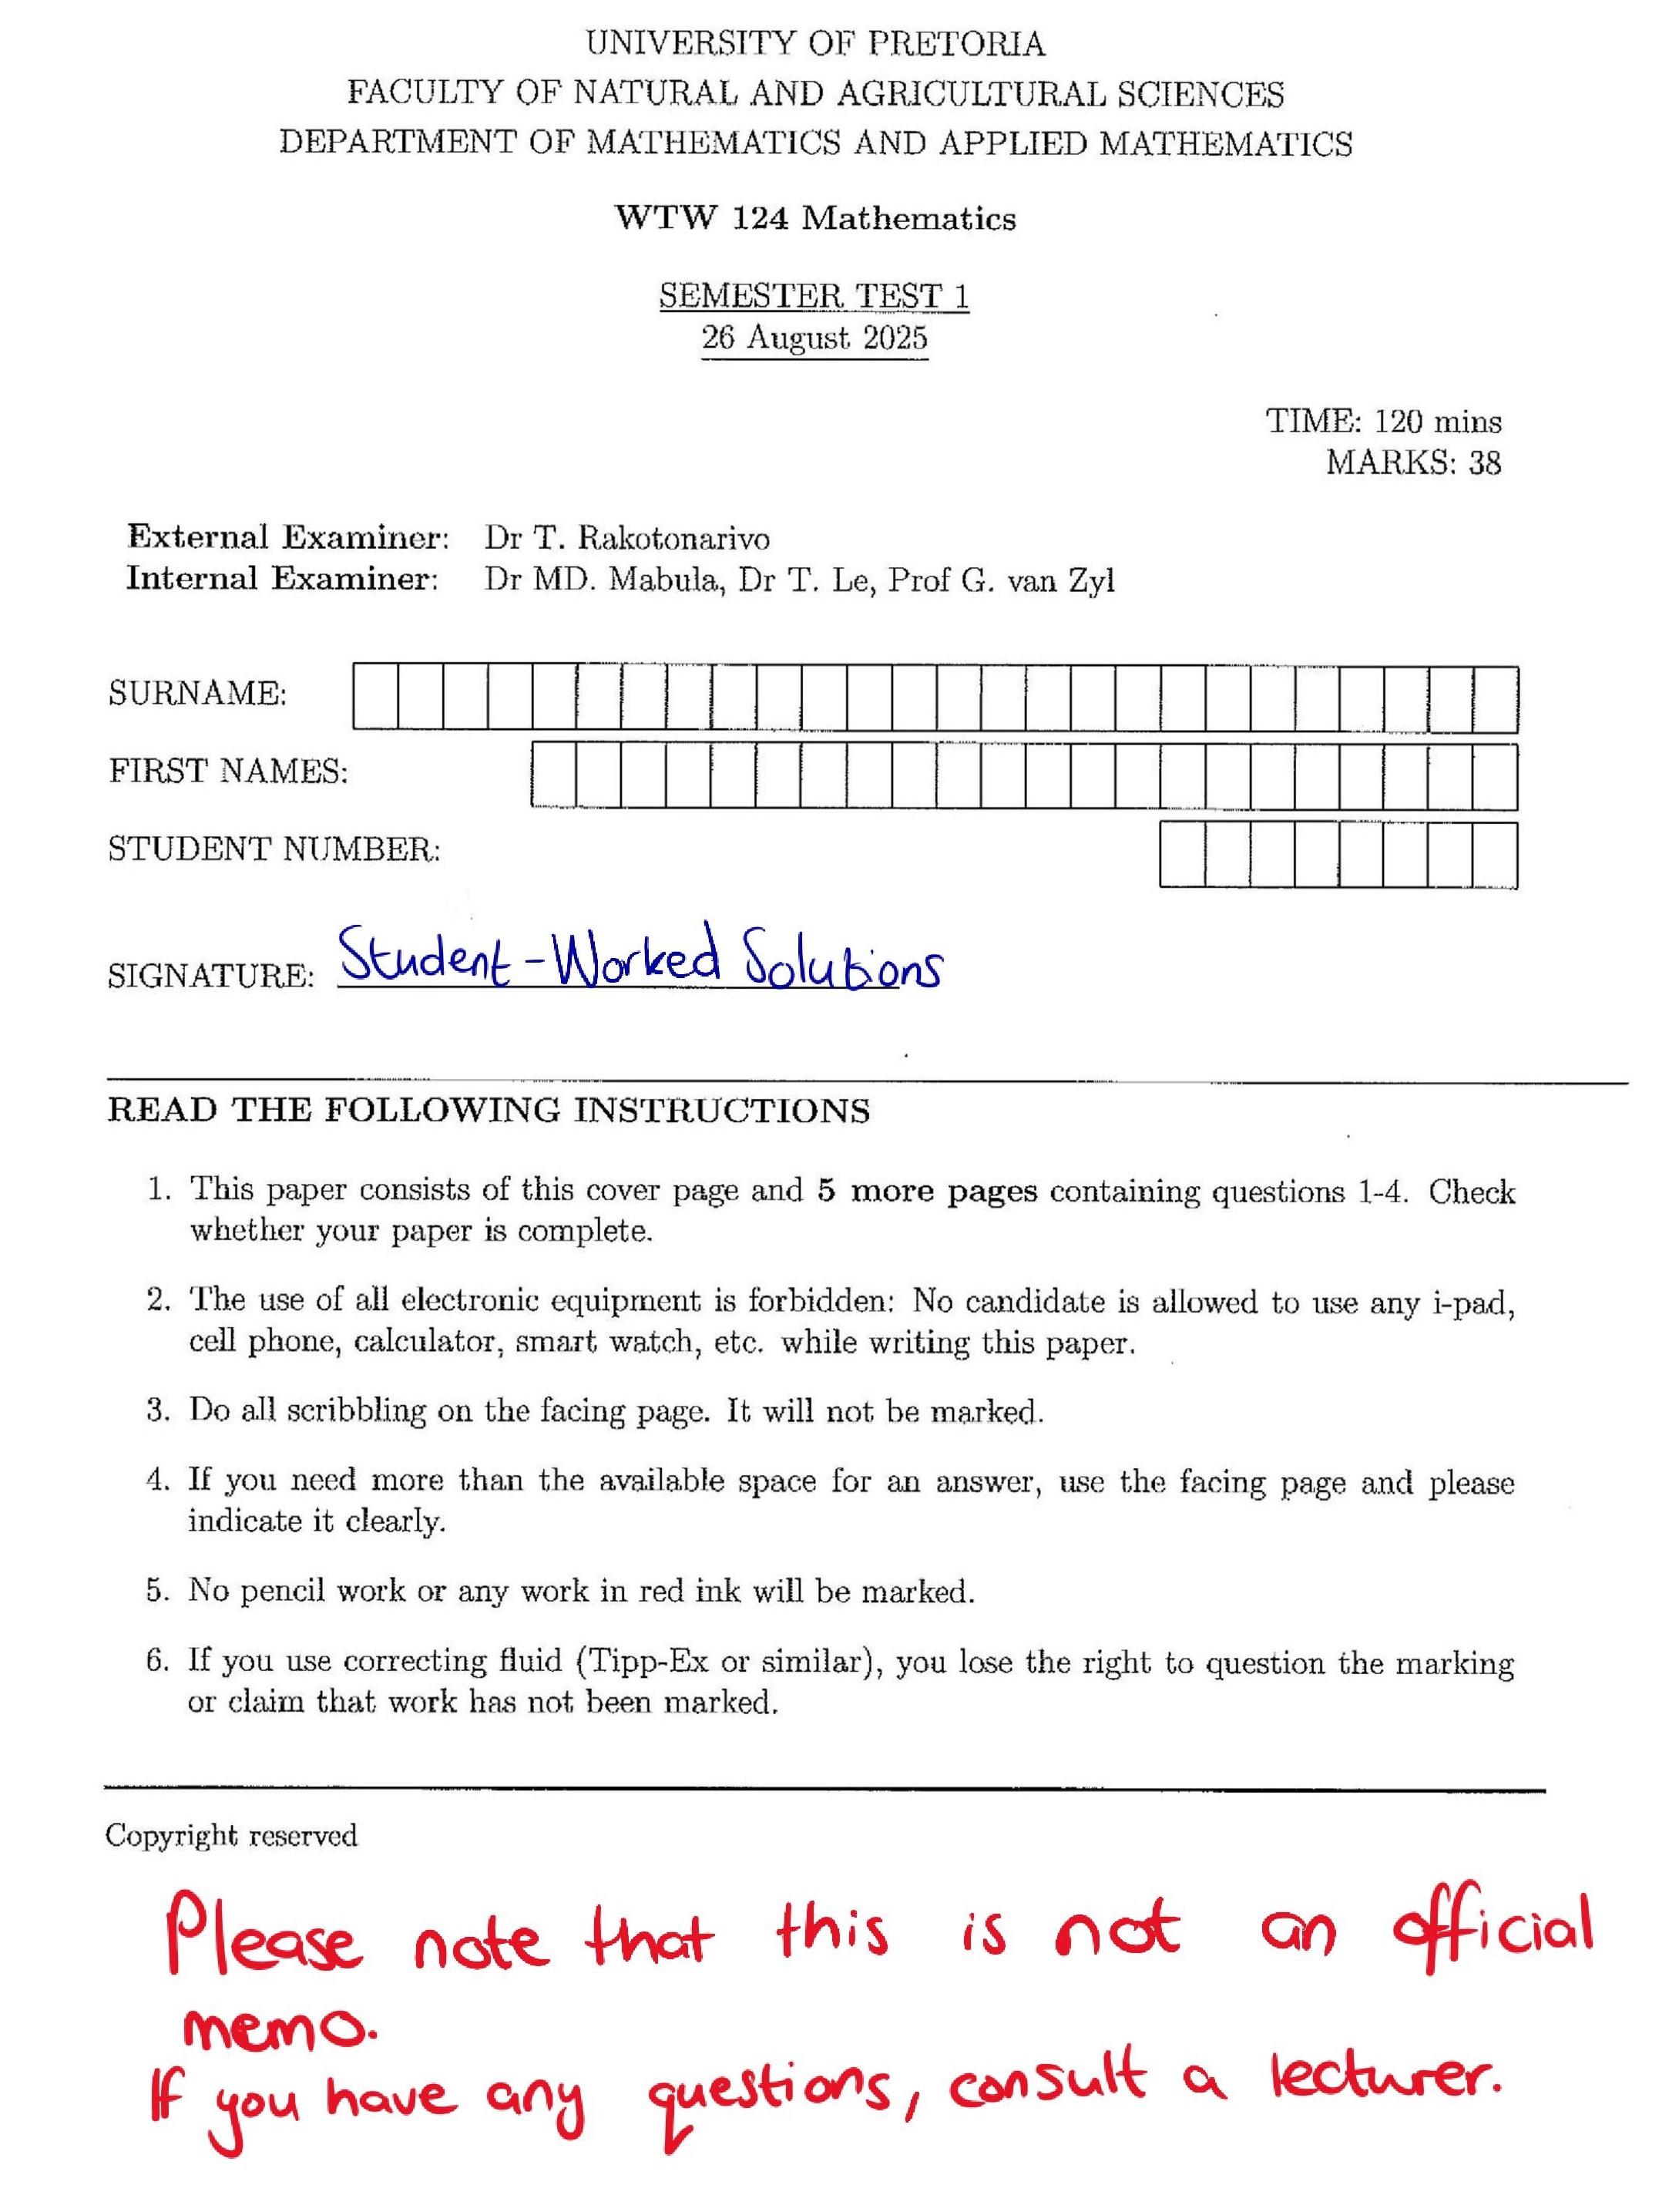
\includegraphics[width=1\textwidth]{TitleMemo.jpg}
\end{figure}

\newpage

\textbf{Question 1.}
\begin{enumerate}[label=\alph*)]
    \item Find two unit vectors perpendicular to both vectors \(\bar{u} =\langle1,2,-1\rangle\) and \(\bar{v}=\langle3,1,2\rangle\). \hfill [3]
    
    \color{blue}
    Any vector perpendicular to both \(\bar{u}\) and \(\bar{v}\) is perpendicular to the vector given by
    \[
        \begin{aligned}
            \bar{u} \times \bar{v} &= \langle1,2,-1\rangle\times\langle3,1,2\rangle\\
            &=\langle4-(-1),-3-2,1-6\rangle\\
            &=\langle5,-5,-5\rangle.
        \end{aligned}
    \]
    Then \(\|\langle5,-5,-5\rangle\| = \sqrt{5^2+(-5)^2+(-5)^2} = 5\sqrt{3}\), so two unit vectors perpendicular to both \(\bar{u}\) and \(\bar{v}\) are
    \[
    \begin{aligned}
      &\frac{1}{5\sqrt{3}}\langle5,-5,-5\rangle = \frac{1}{\sqrt{3}}\langle1,-1,-1\rangle = \langle\frac{1}{\sqrt{3}},-\frac{1}{\sqrt{3}},-\frac{1}{\sqrt{3}}\rangle\\
        &\text{and } -\frac{1}{5\sqrt{3}}\langle5,-5,-5\rangle = -\frac{1}{\sqrt{3}}\langle1,-1,-1\rangle = \langle-\frac{1}{\sqrt{3}},\frac{1}{\sqrt{3}},\frac{1}{\sqrt{3}}\rangle.  
    \end{aligned}
        \]
    \color{black}

    \item Let \(\bar{u}\) and \(\bar{v}\) be two non-zero vectors such that \(\bar{u} \cdot  \bar{v} = \|\bar{u} \times \bar{v}\|\).
    Find the magnitude of the angle between the rays determined by \(\bar{u}\) and \(\bar{v}\) \hfill [3]

    \color{blue}
    We have that \[\cos\theta = \frac{\bar{u} \cdot \bar{v}}{\|\bar{u}\|\|\bar{v}\|}\ \text{ and } \sin\theta = \frac{\|\bar{u} \times \bar{v}\|}{\|\bar{u}\|\|\bar{v}\|},\] where \(\theta\) is the angle between the rays determined by \(\bar{u}\) and \(\bar{v}\).

   Then
   \[
        \cos\theta = \frac{\|\bar{u} \times \bar{v}\|}{\|\bar{u}\|\|\bar{v}\|} = \sin\theta \implies \tan\theta = 1 \implies \theta = \frac{\pi}{4}.
   \]
    \color{black}
    \item Let \(A\), \(B\) and \(C\) be three matrices such that \(ABC\) exists, where \(A\) has size \(3\times3\) and \(C\) has size \(5\times5\).
    Describe the sizes \(B\) and \(ABC\). \hfill [2]

    \color{blue}

    By the associative property of matrix multiplication, we have that \(ABC = (AB)C\).
    
    Since \(ABC\) exists, then \(AB\) must have size \(3\times5\) (because \(C\) has size \(5\times5\)). 
    
    This means that \(B\) must have size \(3\times5\) (because \(A\) has size \(3\times3\)).

    Therefore, \(ABC\) has size \(3\times5\).
    \color{black}
\end{enumerate}

\newpage

\textbf{Question 2.}
\begin{enumerate}[label=\alph*)]
    \item Let \(\bar{u}\) and \(\bar{v}\) be vectors in \(\mathbb{R}^3\). Prove that if \(\bar{u}+\bar{v} = \bar{0}\), then \(\bar{u}\times\bar{v} = \bar{0}\). \hfill [3]
    
    \color{blue}
    Assume \(\bar{u}+\bar{v} = \bar{0}\). Then by the properties of vector addition, we have that \(\bar{v} = (-\bar{u})\), such that
    \[
        \bar{u} + \bar{v} = \bar{u} + (-\bar{u}) = \bar{0}.
    \]
    Then \(\bar{u}\times\bar{v}\) = \(\bar{u}\times(-\bar{u})\).

    Since \(\bar{u}\) and \(\bar{v}\) are scalar multiples of each other, it follows from the properties of the cross product that

    \[
            \bar{u}\times\bar{v} = \bar{u}\times(-\bar{u}) = \bar{0}.    
    \]
    \color{black}
    \item Let \(A\) be a \(2\times2\) matrix. If \(A(A-I) = 0\), then \(A = 0 \text{ or } A = I\); prove or disprove. \hfill [3]
    
    \color{blue}
    For instance, let
    \[
        A = \begin{bmatrix}
            1 & 1\\
            0 & 0
        \end{bmatrix}.
    \]
    Then \(A \neq 0 \text{ and } A \neq I\).

    We have:
        \[
        \begin{aligned}
            A(A-I) &= \begin{bmatrix}
            1 & 1\\
            0 & 0
        \end{bmatrix}
        \left(\begin{bmatrix}
            1 & 1\\
            0 & 0
        \end{bmatrix} - \begin{bmatrix}
            1 & 0\\
            0 & 1
        \end{bmatrix}\right)\\  
        &=\begin{bmatrix}
            1 & 1\\
            0 & 0
        \end{bmatrix}\begin{bmatrix}
            0 & 1\\
            0 & -1
        \end{bmatrix}\\
        &= \begin{bmatrix}
            0 & 1-1\\
            0 & 0
        \end{bmatrix} = \begin{bmatrix}
            0 & 0\\ 0&0
        \end{bmatrix} = 0.
        \end{aligned} 
    \]
    Therefore the claim is false.

    \color{black}

    \item Let \(A\) and \(B\) be \(n\times n\) matrices. Prove that if \(AB = BA\), then \(A^T\) commutes with \(B^T\). \hfill [3]
    \color{blue}

    Assume that \(AB = BA\).
    We show that \(A^TB^T = B^TA^T\)
    \[
        \begin{aligned}
            A^TB^T &= (BA)^T  \qquad &[\text{Properties of the transpose}]\\
            &=(AB)^T \qquad &[\text{By assumption}]\\
            &=B^TA^T    \qquad &[\text{Properties of the transpose}]
        \end{aligned}
    \]
    \color{black}
\end{enumerate}

\newpage

\textbf{Question 3.}
\begin{enumerate}[label=\alph*)]
    \item Use Gaussian elimination to find (if possible) conditions on real numbers \(a\) such that the following system of linear equations
    has no solution: \hfill [4]

    \[ x + ay - z = 1\]
    \[ -x + (a-2)y + z = -1\]
    \[ 2x + 2y + (a-2)z = 1\]
    
    \color{blue}
    We write the system as an augmented matrix and apply Gaussian elimination:

    \[
    \begin{aligned}
        &\left[
            \begin{array}{ccc|c}
                1 & a & -1 & 1\\
                -1 & a-2 & 1 & -1\\
                2 & 2 & a-2 & 1
            \end{array}
        \right] \sim
        \left[
            \begin{array}{ccc|c}
                1 & a & -1 & 1\\
                0 & 2a-2 & 0 & 0\\
                2 & 2 & a-2 & 1
            \end{array}
        \right]
        \left(
            \begin{array}{c}
             R_2 + R_1 \rightarrow R_2\\
            R_3 - 2R_1 \rightarrow R_3   
            \end{array}
        \right) \\
        &\sim
        \left[
            \begin{array}{ccc|c}
                1 & a & -1 & 1\\
                0 & 2a-2 & 0 & 0\\
                0 & 0 & a & -1
            \end{array}
        \right]
        \left(
            R_3 + R_2 \rightarrow R_3
        \right)
        \end{aligned}
    \]

    Now if \(a = 0\), then the third row implies that \(0 = -1\), which is false.\\
    Therefore, by the theorem on the consistency of a system of linear equations,
    the system does not have a solution when \(a = 0\).
    \color{black}
    \item Consider the following matrices:
    \[
A = \begin{bmatrix}
1 & -2 & 2 \\
2 & 1 & 1 \\
1 & 0 & 1
\end{bmatrix}
\text{ and } 
B = \begin{bmatrix}
    1 & 2 & -4 \\
    -1 & -1 & 3 \\
    -1 & -2 & 5
\end{bmatrix}.
\]

Do \(A\) and \(B\) commute? Show all steps. \hfill [3]

\color{blue}
Note that \(A\) and \(B\) both have size \(3\times 3\). Hence \(AB\) and \(BA\) both exist as \(3\times 3\) matrices.
\[ \begin{aligned}
    AB &= \begin{bmatrix}
1 & -2 & 2 \\
2 & 1 & 1 \\
1 & 0 & 1
\end{bmatrix}\begin{bmatrix}
    1 & 2 & -4 \\
    -1 & -1 & 3 \\
    -1 & -2 & 5
\end{bmatrix} \\[1em] 
&= 
\begin{bmatrix}
\langle 1, -2, 2 \rangle \cdot \langle 1,-1,-1 \rangle & \langle 1, -2, 2 \rangle \cdot \langle 2,-1,-2 \rangle & \langle 1, -2, 2 \rangle \cdot \langle -4,3,5 \rangle \\
\langle 2, 1, 1 \rangle \cdot \langle 1,-1,-1 \rangle & \langle 2, 1, 1 \rangle \cdot \langle 2,-1,-2 \rangle & \langle 2, 1, 1 \rangle \cdot \langle -4,3,5 \rangle \\
\langle 1, 0, 1 \rangle \cdot \langle 1,-1,-1 \rangle & \langle 1, 0, 1 \rangle \cdot \langle 2,-1,-2 \rangle & \langle 1, 0, 1 \rangle \cdot \langle -4,3,5 \rangle
\end{bmatrix}\\[1em]
&= \begin{bmatrix}
    1+2-2 & 2+2-4 & -4-6+10\\
    2-1-2 & 4-1-2 & -8+3+5\\
    1-1 & 2-2 & -4+5
\end{bmatrix} = \begin{bmatrix}
1 & 0 & 0 \\
0 & 1 & 0 \\
0 & 0 & 1
\end{bmatrix} = I
\end{aligned}
\]

\[
\begin{aligned}
BA &= 
\begin{bmatrix}
1 & 2 & -4 \\
-1 & -1 & 3 \\
-1 & -2 & 5
\end{bmatrix}
\begin{bmatrix}
1 & -2 & 2 \\
2 & 1 & 1 \\
1 & 0 & 1
\end{bmatrix} \\[1em]
&=
\begin{bmatrix}
\langle 1, 2, -4 \rangle \cdot \langle 1, 2, 1 \rangle & \langle 1, 2, -4 \rangle \cdot \langle -2, 1, 0 \rangle & \langle 1, 2, -4 \rangle \cdot \langle 2, 1, 1 \rangle \\
\langle -1, -1, 3 \rangle \cdot \langle 1, 2, 1 \rangle & \langle -1, -1, 3 \rangle \cdot \langle -2, 1, 0 \rangle & \langle -1, -1, 3 \rangle \cdot \langle 2, 1, 1 \rangle \\
\langle -1, -2, 5 \rangle \cdot \langle 1, 2, 1 \rangle & \langle -1, -2, 5 \rangle \cdot \langle -2, 1, 0 \rangle & \langle -1, -2, 5 \rangle \cdot \langle 2, 1, 1 \rangle
\end{bmatrix} \\[1em]
&=
\begin{bmatrix}
1 + 4 - 4 & -2 + 2 + 0 & 2 + 2 - 4 \\
-1 - 2 + 3 & 2 - 1 + 0 & -2 - 1 + 3 \\
-1 - 4 + 5 & 2 - 2 + 0 & -2 - 2 + 5
\end{bmatrix} \\[1em]
&=
\begin{bmatrix}
1 & 0 & 0 \\
0 & 1 & 0 \\
0 & 0 & 1
\end{bmatrix} = I
\end{aligned}
\]
By the definition of matrix equality, \(AB = BA\), and \(A\) therefore commutes \(B\).

\end{enumerate}
\color{black}

\textbf{Question 4.}

Consider the following two lines in \(\mathbb{R}^3\):
    \[
        L_1 = \{\langle1,2,-3\rangle + t\langle1,2,-3\rangle : t \in \mathbb{R}\}
        \text{ and }
        L_2 = \{\langle-3,1,0\rangle + t\langle-2,4,-6\rangle : t \in \mathbb{R}\}.
    \]
\begin{enumerate}[label=\alph*), series=Last]
    \item If \(P\) is a plane with equation \(2x-y-z=3\), then \(L_1 \subseteq P\).\\
    Is this statement true or false? Explain with full details. \hfill [3]

    \color{blue}
    \(P\) has normal vector \(\bar{n} = \langle 2,-1,-1\rangle\) and \(L_1\) has direction vector \(\bar{d} = \langle 1,2,-3\rangle\).\\
    Then \(\bar{n} \cdot \bar{d} \neq 0\), by the properties of the dot product. By definition of parallelism, \(\bar{n} \nparallel  \bar{d}\), and
    so by the theorem on the relationship between a plane and a line, \(L_1\) and \(P\) intesect in at least one point.

    Let \(\bar{y} \in L_1\) be a point where \(t= 0\).\\
    Then \(\bar{y} = \langle1,2,-3\rangle\)
    We have \(2 -  2- (-3) = 3\). Therefore \(\bar{y} \in P\).

    \vspace{0.5em}
    Let \(\bar{x} \in L_1\) be a point where \(t = 1\).\\
    Then \(\bar{x} = \langle2,4,-6\rangle.\)
    We have \( 2(4) -4 + 6 = 10 \neq 3\). Hence \(\bar{x} \notin P\). 
    
    \vspace{0.5em}
    Therefore \(L_1 \nsubseteq P\). The claim is false.

    \color{black}

    \item Give Cartesian equations for two parallel lines, each containing one of the lines above. \hfill [4]
    \color{blue}

    \(L_1\) has direction vector \(\bar{d_1} = \langle1,2,-3\rangle\), and \(L_2\) direction vector \(\bar{d_2} = \langle-2,4,-6\rangle\).

    Let \(P_1,P_2\) be planes containing \(L_1\) and \(L_2\) respectively.\\
    We know that \(P_1\parallel P_2\) if their normal vectors are parallel to each other.

    \vspace{1em}

    So we need \(\bar{n}\) such that \(\bar{n} \perp \bar{d_1}\) and \(\bar{n} \perp \bar{d_2}\). \hfill {\color{red} [Sketch it if you need to!]}
    \[
        \begin{aligned}
            \bar{n} &= \bar{d_1} \times \bar{d_2} \\
            &= \langle -12+12,6-(-6),4+4 \rangle\\
            &= \langle 0, 12, 8 \rangle
        \end{aligned}
    \]
    \(P_1\) has equation
    \[
        \begin{aligned}
            &\langle 0, 12, 8 \rangle \cdot \left(\langle x,y,z\rangle - \langle 1,2,-3\rangle\right) = 0\\
            &\Rightarrow \langle 0, 12, 8 \rangle \cdot \langle x-1,y-2,z+3\rangle = 0\\
            &\Rightarrow 12y-24+8z+24 = 0 \Rightarrow 12y+8z = 0 \Rightarrow 3y + 2z = 0.
        \end{aligned}
    \]
    \(P_2\) has equation
    \[
        \begin{aligned}
            &\langle 0, 12, 8 \rangle \cdot \left(\langle x,y,z\rangle - \langle -3,1,0\rangle\right) = 0\\
            &\Rightarrow \langle 0, 12, 8 \rangle \cdot \langle x+3, y-1, z \rangle = 0\\
            &\Rightarrow 12y -12 +8z = 0 \Rightarrow 12y + 8z = -2 \Rightarrow 3y + 2z = 3
        \end{aligned}
    \]
    \color{black}

    \item Let \(L\) be a line passing through the point \(\bar{p} = \langle2,0,0\rangle\) such that \(L\) is
    perpendicular to the line \(L_2\) at their intersection. Find a vector equation of the line \(L\). \hfill [4]
    
    \color{blue}
    \(L_2\) has equation \(\bar{x} = \langle-3,1,0\rangle + t\langle-2,4,-6\rangle \) for some \(t \in \mathbb{R}\).\\
    Recall that \(L_2\) has direction vector \(\bar{d_2} = \langle-2,4,-6\rangle\). We want to find \(\bar{d_3} = \langle x,y,z\rangle\) as the direction vector 
    of the unknown line \(L\).
    \[
        \begin{aligned}
            L_2 \perp L &\Rightarrow \bar{d_2} \cdot \bar{d_3} = 0\\
            &\Rightarrow\langle-2,4,-6\rangle \cdot \langle x,y,z\rangle =0\\
            &\Rightarrow -2x+4y-6z = 0
        \end{aligned}
    \]
    \[
    \text{Pick } x = 1 \text{ and } y = 0 \implies -2-6z = 0 \implies -6z = 2 \implies z = -\frac{1}{3}
    \]
    Then \(\bar{d_3} = \langle 1,0, -\frac{1}{3} \rangle\).\\
    Therefore \(L\) has vector equation
    \[
    \bar{x} = \langle 2,0,0 \rangle + t\langle 1,0, -\frac{1}{3} \rangle \text{ for some } t \in \mathbb{R}.\]
    \color{black}
    \item Find the equation of the line through the point \(\bar{p} = \langle2,-1,4\rangle\) and perpendicular to the
    plane\\ \(3x-2y-z=0\). \hfill [3]

    \color{blue}
    Let \(Q\) be a plane with the equation \(3x-2y-z=0\). Then \(Q\) has normal vector \(\bar{m} = \langle 3,-2,-1\rangle\).\\
    Let \(L\) be the line through \(\bar{p}\) with direction vector \(\bar{d}\).

    \vspace{1em}

    \(L, P\) must be such that \(L \perp P\), so it must be the case that \(\bar{d} \parallel\bar{n}\).\\ Let \(\bar{d} = 2\bar{m}\). Then by definition,
    \(\bar{d}\parallel\bar{m}\), and furthermore \(L\perp Q\)!

    Then an equation that satisfies this is:
    \[
    L = \{\langle 2,-1,4\rangle + t\langle 6,-4,-2\rangle : t \in R\}
    \]
\end{enumerate}

\begin{remarkbox}
    These questions need a lot of geometric interpretation. If all fails in the test, \textbf{sketch a picture!}
\end{remarkbox}

\end{document}